% !TEX root =  master.tex
\cleardoublepage
\section{Methoden für PCR-Pooling}
\subsubsection{Minipool}
Das einfachste Verfahren für Pooling ist, eine Serie von N Proben zu verwenden und vor der PCR-Analyse zu kombinieren.
Die Matrix lässt sich hierbei als 1xN beschreiben.
Die Proben werden gemeinsam getestet.
Fällt das Ergebnis negativ aus, wurde mit einem Test festgestellt, dass N Personen negativ sind.
Die Effizienz liegt somit bei N/1.
Sollte das Ergebnis positiv ausfallen, werden die Personen einzeln nachgetestet.
Im Falle einer Nachtestung werden somit N+1 Tests für N Personen benötigt.
Die Testung erfolgt zweistufig.

Der Erwartungswert für die benötigte Anzahl der Tests lässt sich beschreiben als:

Wenn(Pool Positiv)
Dann -> N+1
Andernfalls -> 1

Der erwartete Testbedarf hängt ab von der Wahrscheinlichkeit, dass der Pool positiv ist.
Dieser lässt sich durch die prozentuale Angabe der Testprävalent ermitteln.

Hieraus ergibt sich:
%Erwartungswert Testbedarf = (P(Positiv) * N+1) + (!P(Positiv) * 1)
%N/((MIN(1;N*Prävalenz)*(N+1))+(1-MIN(1;N*Prävalenz)))

P(PoolPositiv) = $(min\left(1;Poolsize\cdot Pravalenz\right)$

Erwartungswert Personen pro Test =
$\frac{Poolsize}{P(PoolPositiv)\cdot (Poolsize + 1)) + (1 - P(PoolPositiv))}$

\begin{figure}[h]
	\centering
	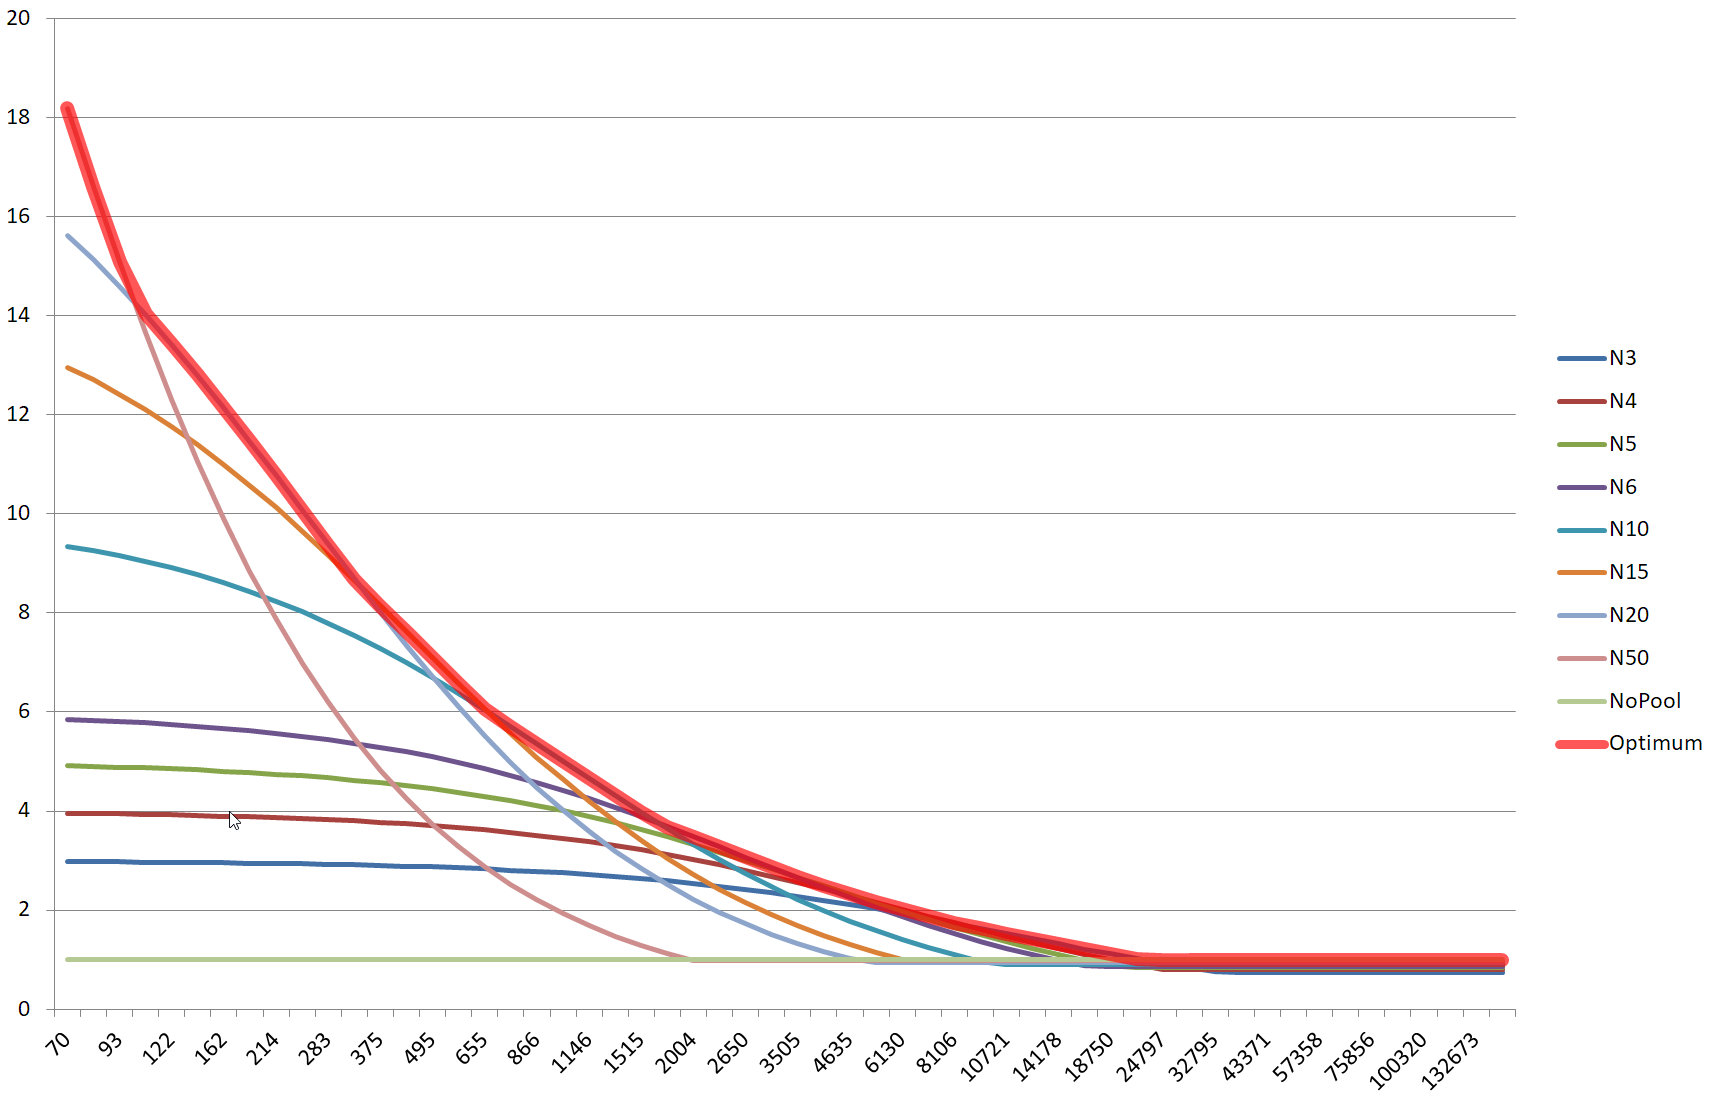
\includegraphics[height=.6\textwidth]{img/Minipool}
	%\caption{Geplanter Aufbau der Arbeit\footnotemark}
\end{figure}

\cleardoublepage
